%
% test_report_v1.tex
%
% Copyright (C) 2021 by SpaceLab.
%
% Documentation of Interstage Interface Panels
%
% This work is licensed under the Creative Commons Attribution-ShareAlike 4.0
% International License. To view a copy of this license,
% visit http://creativecommons.org/licenses/by-sa/4.0/.
%

%
% \brief Test report of the v1.0 hardware.
%
% \author Yan Castro de Azeredo <yan.azeredo@spacelab.ufsc.br>
%
% \institution Universidade Federal de Santa Catarina (UFSC)
%
% \version 0.2.0
%
% \date 2021/07/12
%

\chapter{Test Report of v1.0 Version} \label{anx:test-report-v1}

This appendix is a test report of the first manufactured and assembled PCB (version v1.0).
Only IIP Nº1, Nº2 and Nº3 boards were acquired.

\begin{itemize}
    \item \textbf{PCB manufacturer}: PCBWay (China)
    \item \textbf{PCB assembly}: PCBWay (China)
    \item \textbf{PCB arrival date}: 2021/04/14
    \item \textbf{Execution date}: 2021/04/DD to \textcolor{red}{TBD}
    \item \textbf{Tester}: \textcolor{red}{TBD}
\end{itemize}

\begin{figure}[!ht]
    \begin{center}
        \includegraphics[width=\columnwidth]{figures/v1/iip-n1-top-v1.jpg}
        \caption{Interface Intertage Panel Nº1 top view.}
        \label{fig:iip-n1-v1-top}
    \end{center}
\end{figure}

\begin{figure}[!ht]
    \begin{center}
        \includegraphics[width=\columnwidth]{figures/v1/iip-n1-bottom-v1.jpg}
        \caption{Interface Intertage Panel Nº1 bottom view.}
        \label{fig:iip-n1-v1-bottom}
    \end{center}
\end{figure}

\begin{figure}[!ht]
    \begin{center}
        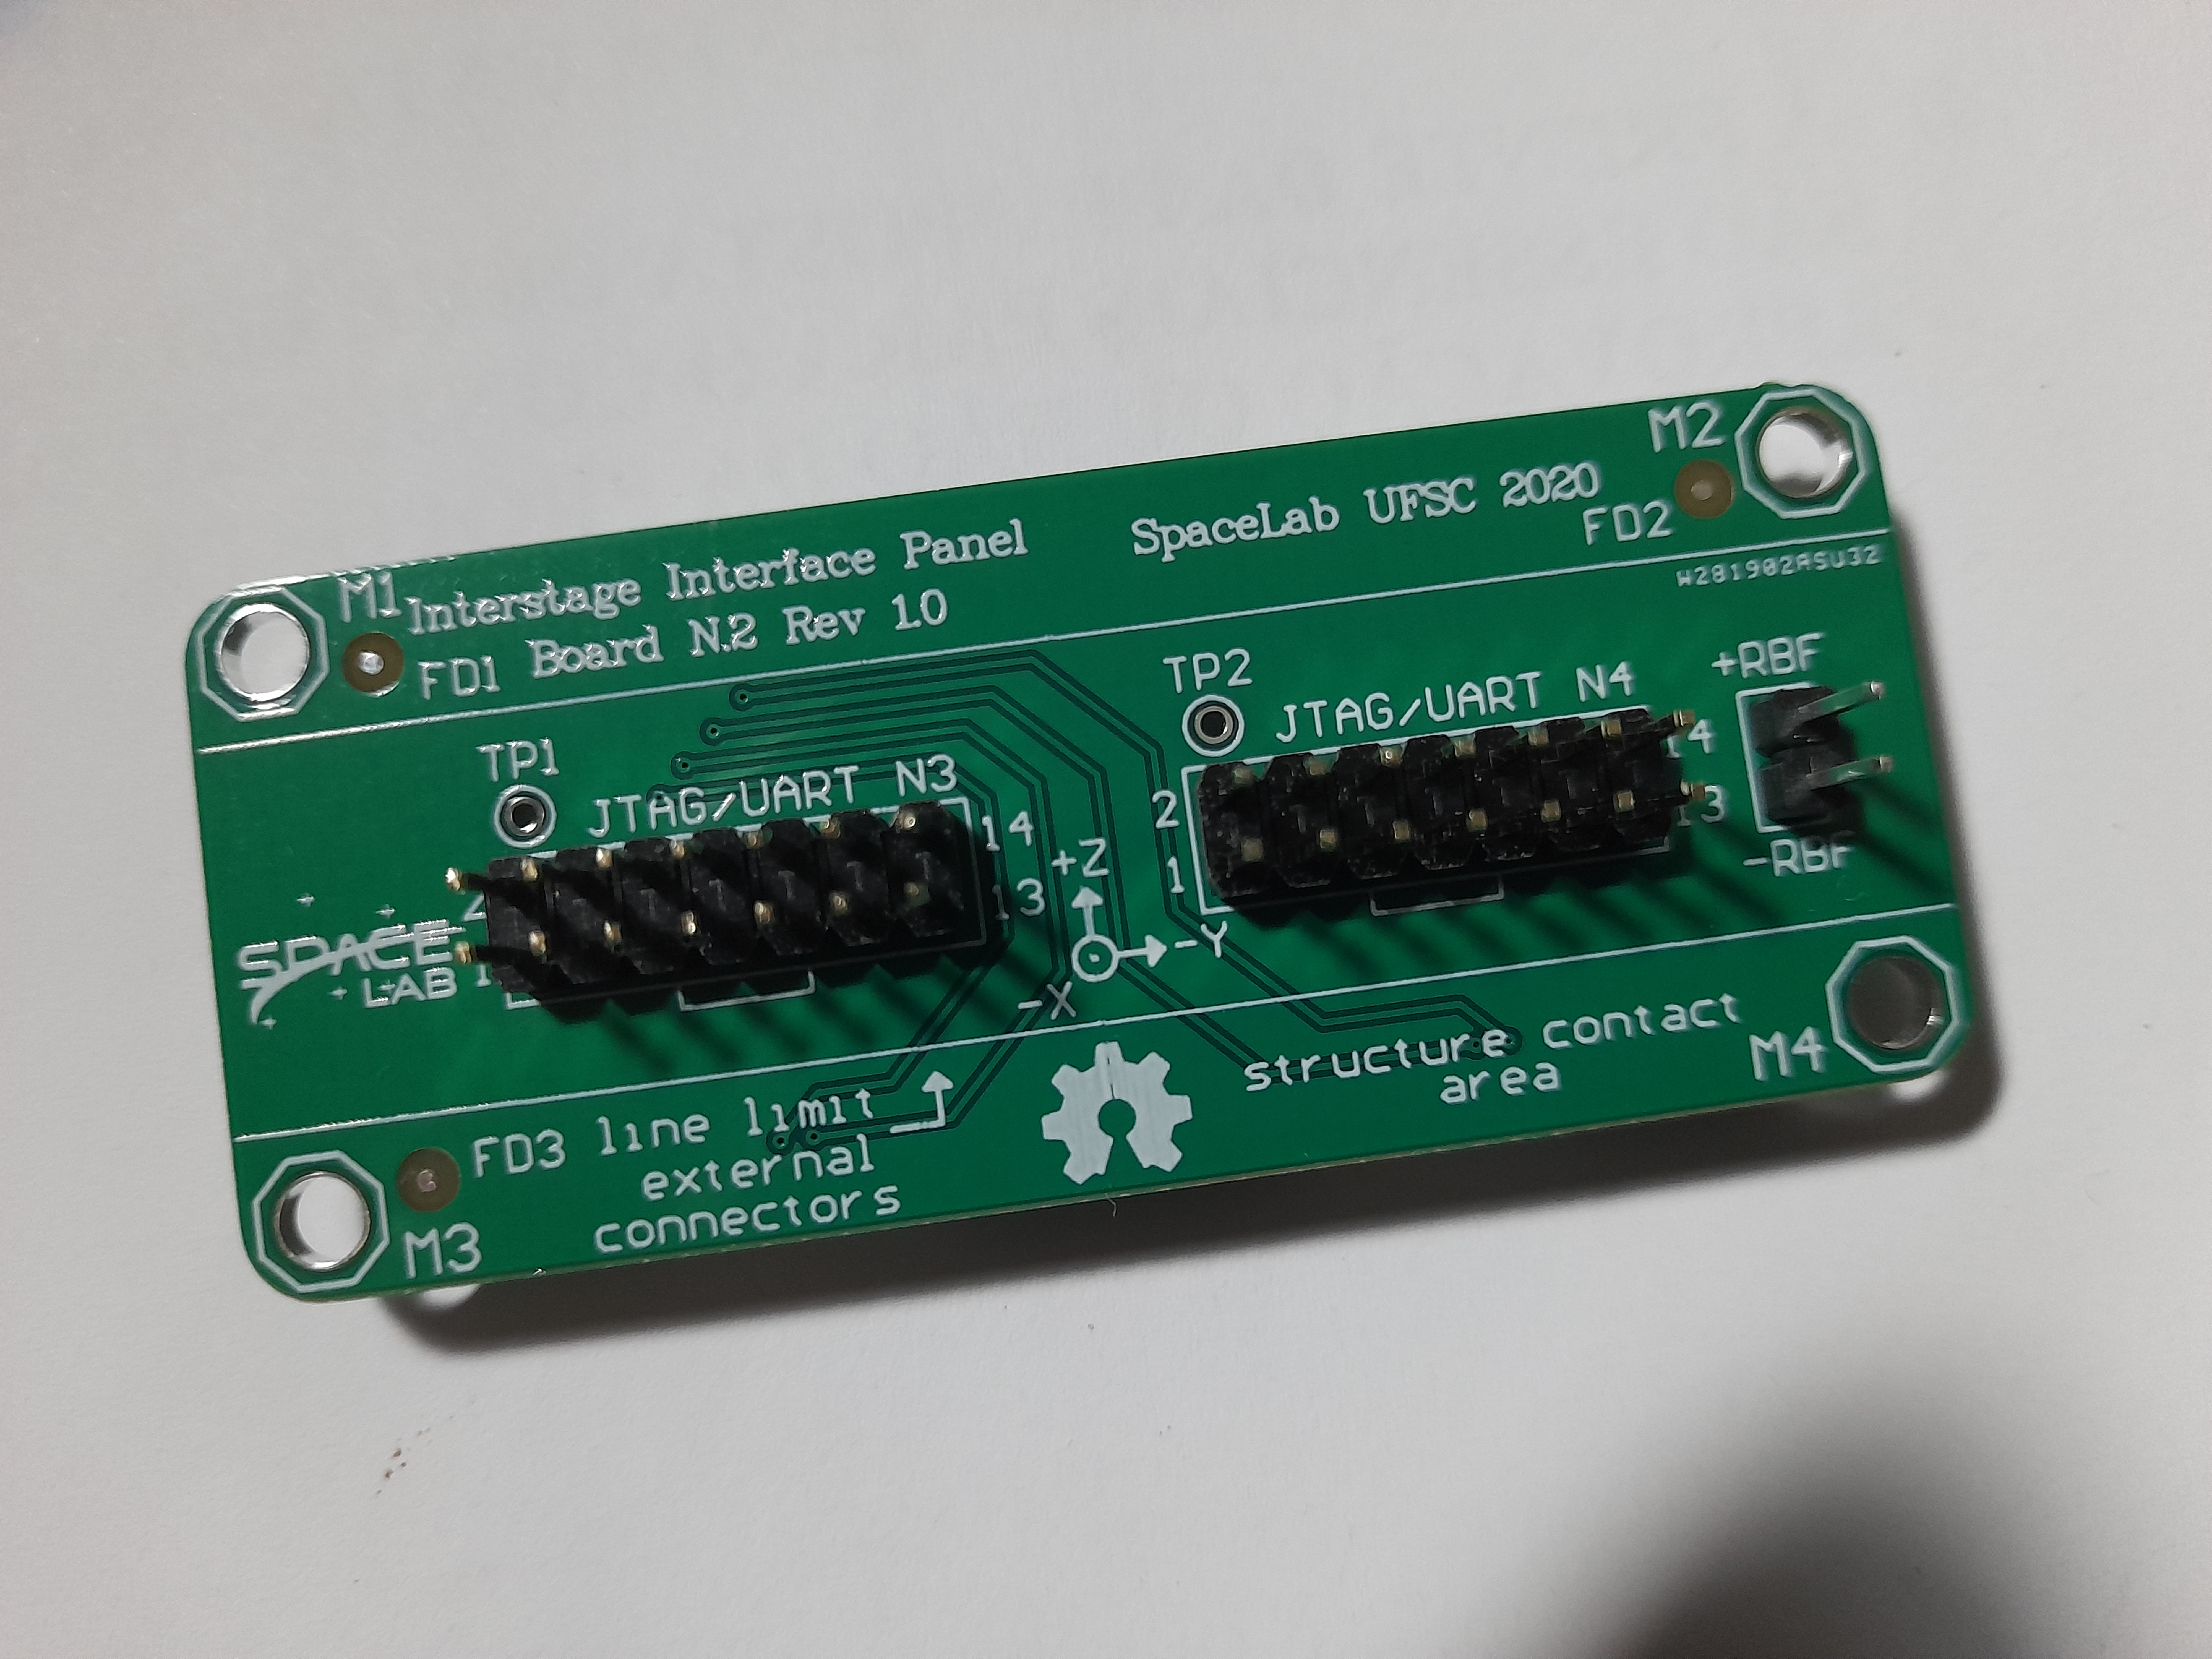
\includegraphics[width=\columnwidth]{figures/v1/iip-n2-top-v1.jpg}
        \caption{Interface Intertage Panel Nº2 top view.}
        \label{fig:iip-n2-v1-top}
    \end{center}
\end{figure}

\begin{figure}[!ht]
    \begin{center}
        \includegraphics[width=\columnwidth]{figures/v1/iip-n2-bottom-v1.jpg}
        \caption{Interface Intertage Panel Nº2 bottom view.}
        \label{fig:iip-n2-v1-bottom}
    \end{center}
\end{figure}

\begin{figure}[!ht]
    \begin{center}
        \includegraphics[width=\columnwidth]{figures/v1/iip-n3-top-v1.jpg}
        \caption{Interface Intertage Panel Nº3 top view.}
        \label{fig:iip-n3-v1-top}
    \end{center}
\end{figure}

\begin{figure}[!ht]
    \begin{center}
        \includegraphics[width=\columnwidth]{figures/v1/iip-n3-bottom-v1.jpg}
        \caption{Interface Intertage Panel Nº3 bottom view.}
        \label{fig:iip-n3-v1-bottom}
    \end{center}
\end{figure}

\section{Visual Inspection}

\begin{itemize}
    \item \textbf{Test description/Objective}: Inspection of the board, visually and with a multimeter, searching for fabrication and assembly failures.
    \item \textbf{Material}:
        \begin{itemize}
            \item Multimeter UNI-T DT830B
        \end{itemize}
    \item \textbf{Results}: \textcolor{red}{TBD}.
    \item \textbf{Conclusion}: \textcolor{red}{TBD}.
\end{itemize}

\section{Mechanical validation}

\begin{itemize}
    \item \textbf{Test description/Objective}: Verify mounting hole sizes, distances, connector heights and silkscreen sinalization. A full assembly of the nanosatellite can be emulated to better test cable managment with connectors positioning.
    \item \textbf{Material}:
        \begin{itemize}
            \item CubeSat 2U or 3U structure 
        \end{itemize}
    \item \textbf{Results}: \textcolor{red}{TBD}.
    \item \textbf{Conclusion}: \textcolor{red}{TBD}.
\end{itemize}

\section{Conclusion}

\textcolor{red}{TBD}
